% !TEX root = ../../../main.tex
% 所属：第二部分：多变量分析学 / 第3章：重积分
% 节：3.2 重积分的性质与计算
% 正文按原文件顺序保存；由 ../chapter3.tex 调用。
\section{重积分的性质与计算}

\subsection*{性质}

除非特别声明，本节所考虑的区域是 $\R^n$（$n\ge2$）中的\textbf{零边界闭区域}。

证明中记 $V$ 为 $\Omega$ 的面积或体积，
$P=\{\Delta\Omega_i\}_{i=1}^N$ 为 $\Omega$ 的划分，
$\Delta V_i$ 为各小块的面积或体积，因而 $\sum_i\Delta V_i=V$。
对有界函数 $u$，记
\[
\omega_i(u)=\sup_{\Delta\Omega_i}u-\inf_{\Delta\Omega_i}u,
\qquad
J_u(P;\xi)=\sum_i u(\vect\xi_i)\Delta V_i,
\quad \vect\xi_i\in\Delta\Omega_i.
\]
前节的 Darboux 和及振幅判据在 $n$ 维情形仍成立：
只需将小块的面积换成体积，将零面积分割边界换成零体积分割边界，
其共同加细与边界邻域估计的证明相同。
以下证明沿用第一部分第八章第四节的方法。

\begin{proposition}[线性性]\label{p2-integral-linearity}
设 $f$ 和 $g$ 都在区域 $\Omega$ 上可积，$\alpha,\beta$ 为常数，
则 $\alpha f+\beta g$ 在 $\Omega$ 上也可积，并且
\[
\int_\Omega(\alpha f+\beta g)\,\dd V
=\alpha\int_\Omega f\,\dd V+\beta\int_\Omega g\,\dd V.
\]
\end{proposition}
\begin{proof}
设 $h=\alpha f+\beta g$。由于 $f,g$ 有界，$h$ 也有界。
对同一小块中的任意两点 $\vect p,\vect q$，有
\[
|h(\vect p)-h(\vect q)|
\le|\alpha|\,|f(\vect p)-f(\vect q)|
+|\beta|\,|g(\vect p)-g(\vect q)|.
\]
取上确界，得到
\[
\omega_i(h)\le|\alpha|\omega_i(f)+|\beta|\omega_i(g).
\]
由 $f,g$ 的可积性，当 $\lambda(P)\to0$ 时，
\[
0\le\sum_i\omega_i(h)\Delta V_i
\le|\alpha|\sum_i\omega_i(f)\Delta V_i
+|\beta|\sum_i\omega_i(g)\Delta V_i\longrightarrow0.
\]
由振幅判据，$h$ 可积。
在同一划分中选取同样的点，则 Riemann 和满足
\[
J_h(P;\xi)=\alpha J_f(P;\xi)+\beta J_g(P;\xi).
\]
令 $\lambda(P)\to0$，由极限的线性性，即得所需积分等式。
\end{proof}

\begin{proposition}[区域可加性]\label{p2-integral-domain-additivity}
设区域 $\Omega$ 被分成两个内部互不相交的区域 $\Omega_1,\Omega_2$。
若 $f$ 在 $\Omega$ 上可积，则 $f$ 在 $\Omega_1,\Omega_2$ 上都可积；
反之，若 $f$ 在 $\Omega_1,\Omega_2$ 上都可积，则 $f$ 在 $\Omega$ 上也可积。
此时成立
\[
\int_\Omega f\,\dd V
=\int_{\Omega_1}f\,\dd V+\int_{\Omega_2}f\,\dd V.
\]
\end{proposition}
\begin{proof}
两个子区域也满足本节的零边界假定。
公共部分包含于 $\partial\Omega_1\cup\partial\Omega_2$ 中，故其面积或体积为零，
划分的面积或体积之和不会因公共边界重复而改变。

必要性：设 $f$ 在 $\Omega$ 上可积。
任给 $\varepsilon>0$，由第二充要条件，可取 $\Omega$ 的划分 $P$，使
\[
\sum_i\omega_i(f)\Delta V_i<\varepsilon.
\]
将 $P$ 的小块分别与 $\Omega_1,\Omega_2$ 相交，得到加细划分 $P^*$。
加细时大和不增、小和不减，故振幅和不增。
将 $P^*$ 限制在 $\Omega_j$ 上，得到 $\Omega_j$ 的划分 $P_j$，
其振幅和只是 $P^*$ 的振幅和中相应的非负部分。因此
\[
\sum_{\Delta E\in P_j}\omega_{\Delta E}(f)\,m(\Delta E)
\le\sum_{\Delta E\in P^*}\omega_{\Delta E}(f)\,m(\Delta E)
\le\sum_i\omega_i(f)\Delta V_i<\varepsilon,
\]
其中 $m(\Delta E)$ 表示小块的面积或体积。
由第二充要条件，$f$ 在 $\Omega_1,\Omega_2$ 上都可积。

充分性：设 $f$ 在 $\Omega_1,\Omega_2$ 上都可积，则它在 $\Omega$ 上有界。
任给 $\varepsilon>0$，分别取两个子区域的划分 $P_1,P_2$，
使各自的振幅和小于 $\varepsilon/2$。
把它们合并为 $\Omega$ 的划分，所得振幅和为两个振幅和之和，
故小于 $\varepsilon$。由第二充要条件，$f$ 在 $\Omega$ 上可积。

最后证明积分等式。分别取子区域的划分 $P_1,P_2$，
并把其中的选点保留到合并后的划分 $P$ 中，则
\[
J_{f,\Omega}(P)
=J_{f,\Omega_1}(P_1)+J_{f,\Omega_2}(P_2),
\qquad
\lambda(P)=\max\{\lambda(P_1),\lambda(P_2)\}.
\]
令两个子区域划分的模长都趋于零，由积分定义及极限的可加性，
即得所需等式。
\end{proof}

\begin{proposition}[常函数的积分]\label{p2-integral-constant}
设被积函数 $f=1$。当 $n=2$ 时，
\[
\iint_\Omega\dd x\,\dd y
=\iint_\Omega1\,\dd x\,\dd y
=\Omega\text{ 的面积；}
\]
当 $n\ge3$ 时，
\[
\int_\Omega\dd V=\int_\Omega1\,\dd V
=\Omega\text{ 的体积。}
\]
\end{proposition}
\begin{proof}
对任意划分及任意选点，都有
\[
J_1(P;\xi)=\sum_i1\cdot\Delta V_i=V.
\]
因此该 Riemann 和的极限就是 $V$，结论成立。
同理，任意常函数 $u\equiv c$ 都可积，且
\[
\int_\Omega c\,\dd V=cV.
\]
这也包括 $V=0$ 的情形。
\end{proof}

\begin{proposition}[保序性]\label{p2-integral-monotonicity}
设 $f$ 和 $g$ 都在区域 $\Omega$ 上可积，且满足 $f\le g$，
则成立
\[
\int_\Omega f\,\dd V\le\int_\Omega g\,\dd V.
\]
\end{proposition}
\begin{proof}
由线性性，$h=g-f$ 可积，并且 $h\ge0$。
任意划分及任意选点所得的 Riemann 和均满足
\[
J_h(P;\xi)=\sum_i h(\vect\xi_i)\Delta V_i\ge0.
\]
令 $\lambda(P)\to0$，得到
\[
0\le\int_\Omega h\,\dd V
=\int_\Omega g\,\dd V-\int_\Omega f\,\dd V.
\]
即得结论。
\end{proof}
\begin{corollary}
	[积分的上下界]\label{p2-integral-bounds}
	设 $f$ 在区域 $\Omega$ 上可积，$M$ 与 $m$ 分别为 $f$ 在 $\Omega$
	上的上界和下界，则
	\[
	mV\le\int_\Omega f\,\dd V\le MV,
	\]
	其中，$n=2$ 时 $V$ 为 $\Omega$ 的面积，$n>2$ 时 $V$ 为 $\Omega$ 的体积。
	这一性质是保序性的直接推论。
\end{corollary}


\begin{proof}
由 $m\le f\le M$，以及常函数的可积性和保序性，有
\[
\int_\Omega m\,\dd V
\le\int_\Omega f\,\dd V
\le\int_\Omega M\,\dd V.
\]
再用常函数的积分公式，即得
$mV\le\displaystyle\int_\Omega f\,\dd V\le MV$。
\end{proof}

\begin{proposition}[绝对可积性]\label{p2-integral-absolute-value}
设 $f$ 在区域 $\Omega$ 上可积，则 $|f|$ 也在 $\Omega$ 上可积，且
\[
\left|\int_\Omega f\,\dd V\right|
\le\int_\Omega|f|\,\dd V.
\]
\end{proposition}
\begin{proof}
对任意 $\vect p,\vect q\in\Omega$，由绝对值不等式，
\[
\bigl||f(\vect p)|-|f(\vect q)|\bigr|
\le|f(\vect p)-f(\vect q)|.
\]
所以在每个小块上，$\omega_i(|f|)\le\omega_i(f)$。
由 $f$ 可积，当 $\lambda(P)\to0$ 时，
\[
0\le\sum_i\omega_i(|f|)\Delta V_i
\le\sum_i\omega_i(f)\Delta V_i\longrightarrow0.
\]
由振幅判据，$|f|$ 可积。
又由 $-|f|\le f\le|f|$，结合线性性与保序性，得到
\[
-\int_\Omega|f|\,\dd V
\le\int_\Omega f\,\dd V
\le\int_\Omega|f|\,\dd V.
\]
这就等价于所需的绝对值不等式。
\end{proof}

\begin{problem}\label{p2-absolute-value-converse-counterexample}
构造一个 $D=[0,1]\times[0,1]$ 上的函数 $f(x,y)$，
使 $|f(x,y)|$ 可积，但 $f(x,y)$ 不可积。
\end{problem}
\begin{solution}
令
\[
f(x,y)=
\begin{cases}
1,&x\in\mathbb Q,\\
-1,&x\notin\mathbb Q,
\end{cases}
\qquad (x,y)\in D.
\]
由于 $|f(x,y)|\equiv1$，由常函数的积分公式，
\[
\iint_D|f(x,y)|\,\dd x\,\dd y=1.
\]
因此 $|f|$ 在 $D$ 上可积。

下面按二重积分的定义证明 $f$ 不可积。
将两个坐标区间都作 $n$ 等分，得到小矩形
\[
\Delta_{ij}=
\left[\frac{i-1}{n},\frac{i}{n}\right]
\times\left[\frac{j-1}{n},\frac{j}{n}\right],
\qquad 1\le i,j\le n.
\]
每个小矩形的面积为 $1/n^2$，
划分的模长为 $\lambda_n=\sqrt2/n\to0$。
由于有理数和无理数在每个非退化区间内都稠密，
每个小矩形中都能选取横坐标为有理数的点，
也能选取横坐标为无理数的点。
若各小矩形中都选前一种点，相应的 Riemann 和为
\[
J_n^+=\sum_{i=1}^n\sum_{j=1}^n1\cdot\frac1{n^2}=1.
\]
若各小矩形中都选后一种点，则
\[
J_n^-=\sum_{i=1}^n\sum_{j=1}^n(-1)\cdot\frac1{n^2}=-1.
\]
两列划分的模长都趋于零，而所得 Riemann 和的极限不同，
故 $f$ 在 $D$ 上不可积。
这个例子说明：$|f|$ 可积不能反推出 $f$ 可积，
即前面绝对可积性命题的逆命题不成立。
\end{solution}

\begin{proposition}[乘积可积性]\label{p2-integral-product}
设 $f$ 和 $g$ 都在区域 $\Omega$ 上可积，则 $f\cdot g$ 也在 $\Omega$ 上可积。
\end{proposition}
\begin{proof}
由于 $f,g$ 有界，可取有限常数 $B_f,B_g\ge0$，使
$|f|\le B_f$、$|g|\le B_g$，因而 $fg$ 也有界。
对同一小块中的任意两点 $\vect p,\vect q$，
\[
\begin{aligned}
|f(\vect p)g(\vect p)-f(\vect q)g(\vect q)|
&\le |f(\vect p)|\,|g(\vect p)-g(\vect q)|\\
&\quad+|g(\vect q)|\,|f(\vect p)-f(\vect q)|\\
&\le B_f|g(\vect p)-g(\vect q)|
+B_g|f(\vect p)-f(\vect q)|.
\end{aligned}
\]
取上确界，得到
\[
\omega_i(fg)\le B_f\omega_i(g)+B_g\omega_i(f).
\]
所以当 $\lambda(P)\to0$ 时，
\[
0\le\sum_i\omega_i(fg)\Delta V_i
\le B_f\sum_i\omega_i(g)\Delta V_i
+B_g\sum_i\omega_i(f)\Delta V_i\longrightarrow0.
\]
由振幅判据，$fg$ 在 $\Omega$ 上可积。
\end{proof}

\begin{proposition}[积分中值定理]\label{p2-integral-mean-value}
设 $f$ 和 $g$ 都在区域 $\Omega$ 上可积，且 $g$ 在 $\Omega$ 上不变号。
设 $M,m$ 分别为 $f$ 在 $\Omega$ 上的上确界和下确界，
则存在常数 $\mu\in[m,M]$，使
\[
\int_\Omega f g\,\dd V=\mu\int_\Omega g\,\dd V.
\]
特别地，若 $f$ 在 $\Omega$ 上连续，且 $\Omega$ 连通，则存在 $\xi\in\Omega$，使
\[
\int_\Omega f g\,\dd V=f(\xi)\int_\Omega g\,\dd V.
\]
\end{proposition}
\begin{proof}
由乘积可积性，$fg$ 可积。
先设 $g\ge0$。由 $m\le f\le M$，有
\[
mg\le fg\le Mg.
\]
根据线性性与保序性，
\[
m\int_\Omega g\,\dd V
\le\int_\Omega fg\,\dd V
\le M\int_\Omega g\,\dd V.
\]
记 $G=\displaystyle\int_\Omega g\,\dd V\ge0$。
若 $G>0$，令
\[
\mu=\frac{\displaystyle\int_\Omega fg\,\dd V}{G},
\]
则上述不等式给出 $m\le\mu\le M$，所需等式成立。
若 $G=0$，上述不等式给出 $\displaystyle\int_\Omega fg\,\dd V=0$，
此时任取 $\mu\in[m,M]$ 都满足所需等式。
若 $g\le0$，对 $-g\ge0$ 使用刚证明的结论，再由线性性同时变号，
就得到关于原函数 $g$ 的结论。

特别地，若 $f$ 连续且 $\Omega$ 连通，
则由于 $\Omega$ 为有界闭集，$f$ 在其上取到最小值 $m$ 和最大值 $M$；
又因连续函数将连通集映为连通集，$f(\Omega)$ 是区间 $[m,M]$。
因此对上述 $\mu\in[m,M]$，存在 $\xi\in\Omega$，使 $f(\xi)=\mu$。
代入前面的等式，便得到
\[
\int_\Omega fg\,\dd V=f(\xi)\int_\Omega g\,\dd V.
\]
若“区域”已按连通集理解，连通性即包含在区域的假定中；
若允许任意零边界闭集，则最后这个取值结论需要另加连通性。
\end{proof}

\subsection*{计算}
\subsubsection*{矩形区域上的二重积分}

对于矩形区域 $D=[a,b]\times[c,d]$（$a\le b$，$c\le d$），
若有一个等号成立，则 $D$ 退化为一段线段，因而
\[
\iint_D f(x,y)\,\dd x\,\dd y=0.
\]
这里仍是二重积分，不等同于沿该线段的一元积分。
若 $a=b$ 且 $c=d$，则 $D$ 退化为一个点，其二重积分同样为零。
以下讨论非退化矩形。

\begin{theorem}[矩形区域上二重积分与累次积分的关系]\label{p2-double-iterated-integral}
设 $f(x,y)$ 在 $D=[a,b]\times[c,d]$ 上可积。
若对每个 $x\in[a,b]$，
\[
h(x)=\int_c^d f(x,y)\,\dd y
\]
都有定义，则 $h$ 在 $[a,b]$ 上可积，并且
\[
\begin{aligned}
\iint_D f(x,y)\,\dd x\,\dd y
&=\int_a^b h(x)\,\dd x\\
&=\int_a^b\left(\int_c^d f(x,y)\,\dd y\right)\dd x
=\int_a^b\dd x\int_c^d f(x,y)\,\dd y.
\end{aligned}
\]
若对每个 $y\in[c,d]$，
\[
g(y)=\int_a^b f(x,y)\,\dd x
\]
都有定义，则 $g$ 在 $[c,d]$ 上可积，并且
\[
\iint_D f(x,y)\,\dd x\,\dd y
=\int_c^d\dd y\int_a^b f(x,y)\,\dd x.
\]
\end{theorem}

\begin{proof}
证明第一种积分次序，另一种同理。
在 $[a,b]$ 上取划分
\[
P_x:\quad a=x_0<x_1<\cdots<x_n=b,
\]
记 $\Delta x_k=x_k-x_{k-1}$，在每个区间 $[x_{k-1},x_k]$
中任取 $\xi_k$。考察 $h$ 的 Riemann 和
\[
\sum_{k=1}^n h(\xi_k)\Delta x_k
=\sum_{k=1}^n\left(\int_c^d f(\xi_k,y)\,\dd y\right)\Delta x_k.
\]
再在 $[c,d]$ 上取划分
\[
P_y:\quad c=y_0<y_1<\cdots<y_m=d,
\qquad \Delta y_j=y_j-y_{j-1}.
\]
两划分给出矩形小块
\[
\Delta_{kj}=[x_{k-1},x_k]\times[y_{j-1},y_j].
\]
令 $m_{kj}=\inf_{\Delta_{kj}}f$，$M_{kj}=\sup_{\Delta_{kj}}f$。
由切片积分的区间可加性及保序性，
\[
\begin{aligned}
R_h(P_x;\xi)
&=\sum_{k=1}^n\sum_{j=1}^m
\left(\int_{y_{j-1}}^{y_j}f(\xi_k,y)\,\dd y\right)\Delta x_k,\\
\sum_{k=1}^n\sum_{j=1}^m m_{kj}\Delta x_k\Delta y_j
&\le R_h(P_x;\xi)
\le\sum_{k=1}^n\sum_{j=1}^m M_{kj}\Delta x_k\Delta y_j.
\end{aligned}
\]
两端分别为该矩形划分的 Darboux 小和与大和。
记 $I=\displaystyle\iint_D f\,\dd x\,\dd y$。由 $f$ 的可积性，
当矩形划分的最大直径趋于零时，两端都趋于 $I$。
具体地，任给 $\varepsilon>0$，可取 $\delta>0$，
使矩形划分的模长小于 $\delta$ 时，两端都与 $I$ 相差小于 $\varepsilon$。
只要 $P_x$ 的模长小于 $\delta/2$，再选 $P_y$ 的模长小于 $\delta/2$，
各矩形的直径就小于 $\delta$，因而对任意 $\xi_k$，
\[
|R_h(P_x;\xi)-I|<\varepsilon.
\]
又因为 $f$ 有界，$h$ 也有界，故按一元 Riemann 积分的定义，
$h$ 在 $[a,b]$ 上可积，且
\[
\int_a^b h(x)\,\dd x=I.
\]
\end{proof}

\textbf{注意：}仅由 $f$ 在矩形上的二重积分存在，
不能推出每个切片积分
$\displaystyle\int_c^d f(x,y)\,\dd y$ 或 $\displaystyle\int_a^b f(x,y)\,\dd x$ 都有定义。

\begin{example}[二重积分存在而某些切片不可积]
设 $D=[0,1]\times[0,1]$。当 $x=q_x/p_x$、$y=q_y/p_y$
都是既约分数时，令
\[
f(x,y)=
\begin{cases}
\dfrac1{p_x}+\dfrac1{p_y},
&x=\dfrac{q_x}{p_x}\in\mathbb Q,\quad
y=\dfrac{q_y}{p_y}\in\mathbb Q,\\[6pt]
0,&\text{其他},
\end{cases}
\]
其中 $p_x,p_y>0$，$(q_x,p_x)=(q_y,p_y)=1$。
此函数在 $D$ 上可积，且
\[
\iint_D f(x,y)\,\dd x\,\dd y=0.
\]

考察切片 $y\mapsto f(x,y)$。
若 $x\notin\mathbb Q$，则此切片恒为零。
若固定 $x=q_x/p_x\in\mathbb Q$，则
\[
f(x,y)=
\begin{cases}
\dfrac1{p_x}+\dfrac1{p_y},&y=\dfrac{q_y}{p_y}\in\mathbb Q,\\[6pt]
0,&y\notin\mathbb Q.
\end{cases}
\]
对 $[0,1]$ 的任意划分，每个子区间的振幅都不小于 $1/p_x$，故
\[
\sum_j\omega_j\Delta y_j
\ge\frac1{p_x}\sum_j\Delta y_j=\frac1{p_x}.
\]
所以该切片不可积，$\int_0^1 f(x,y)\,\dd y$ 没有定义。

二重积分为零可以用第一部分已经定义的 Riemann 函数 $R$ 证明。
仍记
\[
R(t)=
\begin{cases}
1/p,&t=q/p\in[0,1]\cap\mathbb Q,\quad (q,p)=1,\ p>0,\\
0,&t\notin\mathbb Q.
\end{cases}
\]
这里 $[0,1]\cap\mathbb Q$ 表示 $[0,1]$ 内的有理数，
$(q,p)=1$ 表示 $q,p$ 互质，即 $q/p$ 为既约分数。
已知 $R$ 可积且 $\displaystyle\int_0^1R(t)\,\dd t=0$。

分别在两个坐标区间上取一元划分
\[
\begin{aligned}
P_x:&\quad 0=x_0<x_1<\cdots<x_n=1,\\
P_y:&\quad 0=y_0<y_1<\cdots<y_m=1,
\end{aligned}
\qquad
\Delta x_k=x_k-x_{k-1},\quad
\Delta y_j=y_j-y_{j-1}.
\]
由这两组分点组成的矩形划分记为 $P$，其小块仍为
\[
\Delta_{kj}=[x_{k-1},x_k]\times[y_{j-1},y_j].
\]
$P_x\times P_y$ 是这个矩形划分 $P$ 的另一种记法，称为乘积划分。
\[
M_{kj}=\sup_{\Delta_{kj}}f,\qquad
S_f(P)=S(P)=\sum_{k=1}^n\sum_{j=1}^m
M_{kj}\Delta x_k\Delta y_j.
\]
$S_R(P_x)$ 和 $S_R(P_y)$ 则分别是 $R$ 对两个一元划分的 Darboux 大和：
\[
\begin{aligned}
S_R(P_x)
&=\sum_{k=1}^n
\left(\sup_{x\in[x_{k-1},x_k]}R(x)\right)\Delta x_k,\\
S_R(P_y)
&=\sum_{j=1}^m
\left(\sup_{y\in[y_{j-1},y_j]}R(y)\right)\Delta y_j.
\end{aligned}
\]


现在由 $0\le f(x,y)\le R(x)+R(y)$，在每个矩形小块上都有
\[
0\le M_{kj}
\le\sup_{x\in[x_{k-1},x_k]}R(x)
+\sup_{y\in[y_{j-1},y_j]}R(y).
\]
乘以小块面积 $\Delta x_k\Delta y_j$ 后求和。
由于 $\sum_k\Delta x_k=\sum_j\Delta y_j=1$，得到
\[
\begin{aligned}
0\le S(P)
&\le
\sum_{k=1}^n
\left(\sup_{x\in[x_{k-1},x_k]}R(x)\right)\Delta x_k
\sum_{j=1}^m\Delta y_j\\
&\quad+
\sum_{j=1}^m
\left(\sup_{y\in[y_{j-1},y_j]}R(y)\right)\Delta y_j
\sum_{k=1}^n\Delta x_k\\
&=S_R(P_x)+S_R(P_y).
\end{aligned}
\]
因此，原来的简写不等式
\[
0\le S_f(P_x\times P_y)\le S_R(P_x)+S_R(P_y)
\]
就是上述逐块估计的结果。
因为 $R$ 的一元积分为零，当两个一元划分的模长趋于零时，
右边两个 Darboux 大和都趋于零。
又因 $0\le s(P)\le S(P)$，可以取划分使
$S(P)-s(P)$ 任意小。
由二重积分的第二充要条件，$f$ 可积；
再由 $0\le\displaystyle\iint_D f\,\dd x\,\dd y\le S(P)$，得到其积分为零。


\textbf{任意点处的极限是否都为零？}
对于本例的二元函数 $f$，考虑断言
\[
\text{对任意 }(x_0,y_0)\in D,\qquad
\lim_{(x,y)\to(x_0,y_0)}f(x,y)=0.
\]
这一断言是错误的。下面给出反例。

取 $x_0=1/2$、$y_0=\sqrt2/2$，固定 $x=x_0$。
由本例的定义及第一部分示例 6.3.6 中 $R(y)\to0$ 的结论，
\[
\lim_{\substack{y\to y_0\\y\in\mathbb Q}}f(1/2,y)=\frac12,
\qquad
\lim_{\substack{y\to y_0\\y\notin\mathbb Q}}f(1/2,y)=0.
\]
两种趋近方式均符合前面定义的二元去心邻域：
虽然 $x=x_0$，但 $y\ne y_0$，故 $(x,y)\ne(x_0,y_0)$。
所得极限不同，所以 $f$ 在该点的二元极限不存在。

\textbf{与一元 Riemann 函数的比较。}
虽然 $0\le f(x,y)\le R(x)+R(y)$，但按前面的定义，二元去心条件为
$(x,y)\ne(x_0,y_0)$，允许其中一个坐标保持不变。
因此不能把两个一元去心极限直接套用到所有这样的趋近方式上。
若额外限制两个坐标都不等于各自的极限坐标，则可由示例 6.3.6 的方法得到
\[
\lim_{\substack{(x,y)\to(x_0,y_0)\\x\ne x_0,\ y\ne y_0}}f(x,y)=0.
\]
这是一种限制趋近方式后的极限，不能替代通常的二元极限。
对于 $x_0,y_0$ 都为无理数的点，因为 $R(x_0)=R(y_0)=0$，
两个一元估计在坐标等于极限坐标时也成立，
所以由 $0\le f(x,y)\le R(x)+R(y)$ 可知通常的二元极限确实为零。
\end{example}

\subsubsection*{矩形区域上的 $n$ 重积分}

\begin{theorem}
设 $f(x_1,\ldots,x_n)$ 在 $n$ 维闭矩形
\[
\Omega=[a_1,b_1]\times\cdots\times[a_n,b_n]
\]
上可积，记 $\Omega_2=[a_2,b_2]\times\cdots\times[a_n,b_n]$。
若对每个 $x_1\in[a_1,b_1]$，
\[
h(x_1)=\int_{\Omega_2}f(x_1,x_2,\ldots,x_n)\,\dd x_2\cdots\dd x_n
\]
都存在，则 $h$ 在 $[a_1,b_1]$ 上可积，且
\[
\begin{aligned}
\int_\Omega f(x_1,\ldots,x_n)\,\dd x_1\cdots\dd x_n
&=\int_{a_1}^{b_1}h(x_1)\,\dd x_1\\
&=\int_{a_1}^{b_1}\dd x_1
\int_{\Omega_2}f(x_1,\ldots,x_n)\,\dd x_2\cdots\dd x_n.
\end{aligned}
\]
\end{theorem}

特别地，$n=2$ 时就是前面的二重积分定理；
$n=3$ 时，若 $\Omega=[a,b]\times[c,d]\times[e,f]$，
$\Omega_2=[c,d]\times[e,f]$，则
\[
\iiint_\Omega f(x,y,z)\,\dd x\,\dd y\,\dd z
=\int_a^b\dd x\iint_{\Omega_2}f(x,y,z)\,\dd y\,\dd z.
\]

\begin{corollary}
若 $f(x_1,\ldots,x_n)$ 在闭矩形
$\Omega=[a_1,b_1]\times\cdots\times[a_n,b_n]$ 上连续，则
\[
\int_\Omega f\,\dd x_1\cdots\dd x_n
=\int_{a_1}^{b_1}\dd x_1\int_{a_2}^{b_2}\dd x_2\cdots
\int_{a_{n-1}}^{b_{n-1}}\dd x_{n-1}
\int_{a_n}^{b_n}f(x_1,\ldots,x_n)\,\dd x_n.
\]
\end{corollary}

\subsubsection*{一般区域上的重积分计算}

现在考虑 $f(x,y)$ 在一般区域上的二重积分。
设 $f$ 在区域
\[
D=\{(x,y):y_1(x)\le y\le y_2(x),\ a\le x\le b\}
\]
上连续,我们称这样的区域为$x-$区域，其中 $y_1,y_2$ 为 $[a,b]$ 上的一元连续函数。
令
\[
c=\min_{a\le x\le b}y_1(x),\qquad
d=\max_{a\le x\le b}y_2(x),
\qquad
\widetilde D=[a,b]\times[c,d]\supset D.
\]

\begin{center}
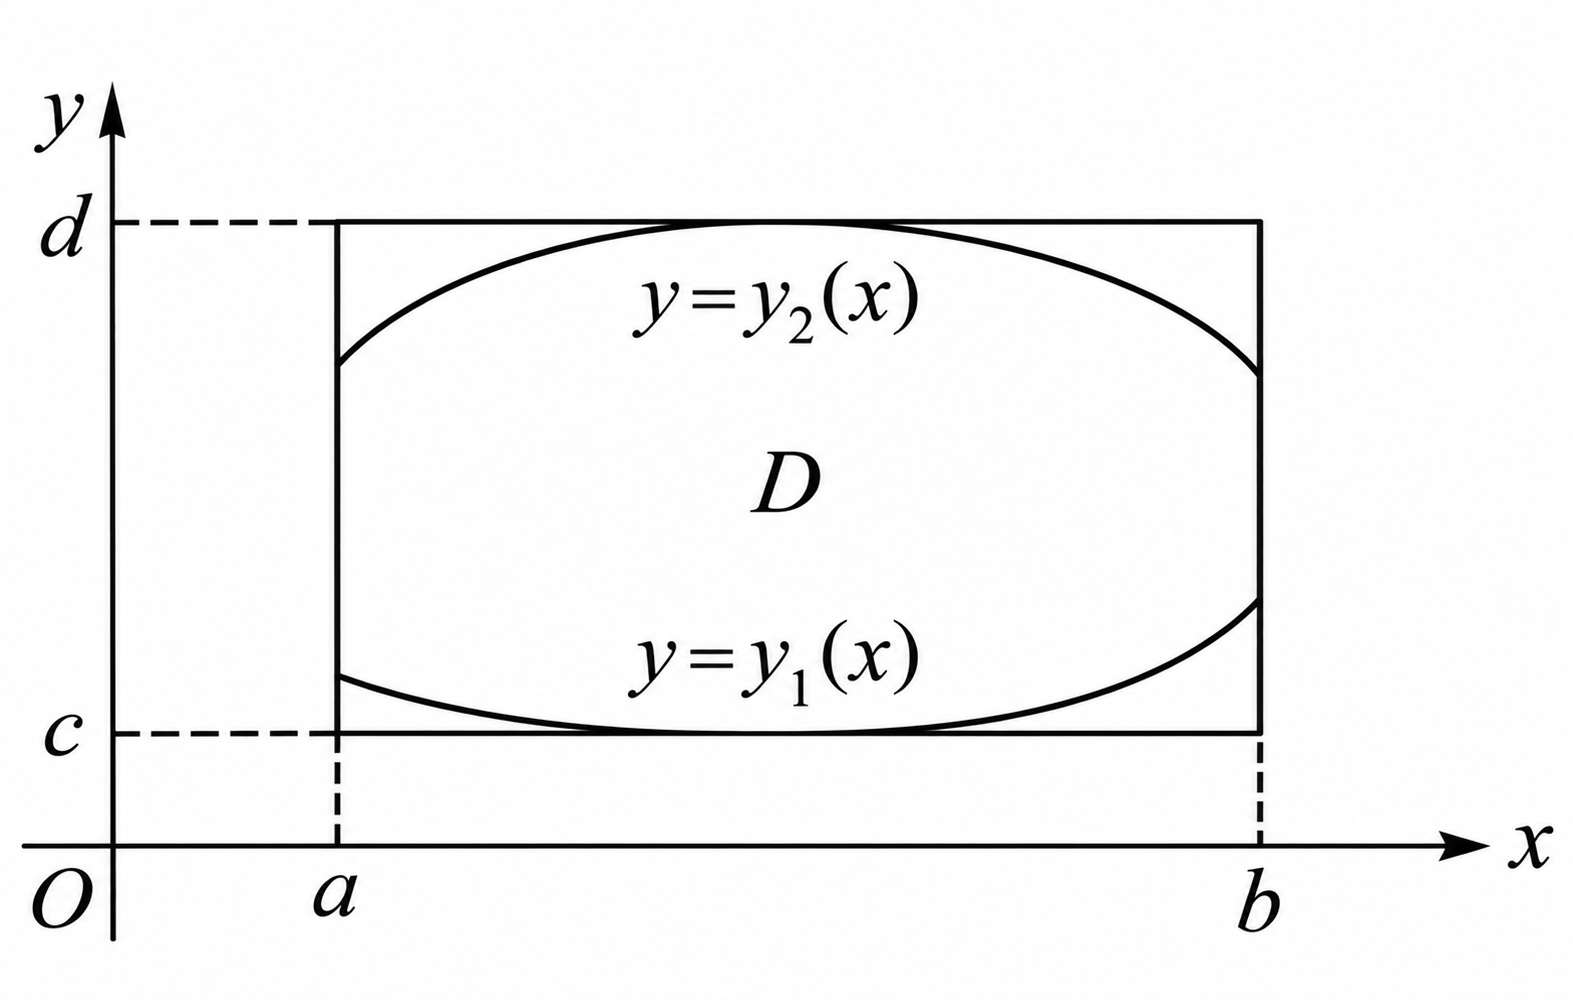
\includegraphics[width=0.5\textwidth]{figure/P2/section2_general_region_hd.png}
\end{center}

令
\[
\widetilde f(x,y)=
\begin{cases}
f(x,y),&(x,y)\in D,\\
0,&(x,y)\in\widetilde D\setminus D.
\end{cases}
\]
$\widetilde f$ 在 $\widetilde D$ 上可积，因为它只可能在零面积边界
$\partial D$ 处不连续。
注意到 $\widetilde f$ 在 $D$ 外为零，对固定的 $x$，
\[
\begin{aligned}
\int_c^d\widetilde f(x,y)\,\dd y
&=\int_c^{y_1(x)}\widetilde f(x,y)\,\dd y
+\int_{y_1(x)}^{y_2(x)}\widetilde f(x,y)\,\dd y
+\int_{y_2(x)}^d\widetilde f(x,y)\,\dd y\\
&=\int_{y_1(x)}^{y_2(x)}f(x,y)\,\dd y.
\end{aligned}
\]
由于 $f$ 在 $D$ 上连续，上式对每个 $x\in[a,b]$ 都有定义。
因此
\[
\begin{aligned}
\iint_D f(x,y)\,\dd x\,\dd y
&=\iint_{\widetilde D}\widetilde f(x,y)\,\dd x\,\dd y\\
&=\int_a^b\dd x\int_c^d\widetilde f(x,y)\,\dd y\\
&=\int_a^b\dd x\int_{y_1(x)}^{y_2(x)}f(x,y)\,\dd y.
\end{aligned}
\]

类似地，若 $f$ 在
\[
D=\{(x,y):x_1(y)\le x\le x_2(y),\ c\le y\le d\}
\]
上连续，且 $x_1,x_2$ 在 $[c,d]$ 上连续，则
\[
\iint_D f(x,y)\,\dd x\,\dd y
=\int_c^d\dd y\int_{x_1(y)}^{x_2(y)}f(x,y)\,\dd x.
\]
\subsubsection*{三重积分}
若积分区域为长方体
\[
D=[a,b]\times[c,d]\times[e,f],
\]
则可以按照前面的累次积分公式计算三重积分。

对于一般区域 $\Omega$，一种方法是投影法，
另一种方法是截面法。

\textbf{投影法：}在三维情形，若 $f(x,y,z)$ 在
\[
\Omega=\{(x,y,z):
z_1(x,y)\le z\le z_2(x,y),\
y_1(x)\le y\le y_2(x),\
a\le x\le b\}
\]
上连续，且 $z_1,z_2,y_1,y_2$ 都连续，则
\[
\begin{aligned}
\iiint_\Omega f(x,y,z)\,\dd x\,\dd y\,\dd z
&=\iint_{\Omega_{xy}}\dd x\,\dd y
\int_{z_1(x,y)}^{z_2(x,y)}f(x,y,z)\,\dd z\\
&=\int_a^b\dd x\int_{y_1(x)}^{y_2(x)}\dd y
\int_{z_1(x,y)}^{z_2(x,y)}f(x,y,z)\,\dd z,
\end{aligned}
\]
其中
\[
\Omega_{xy}=\{(x,y):y_1(x)\le y\le y_2(x),\ a\le x\le b\}
\]
为区域 $\Omega$ 在 $xy$ 平面上的投影。

\begin{center}
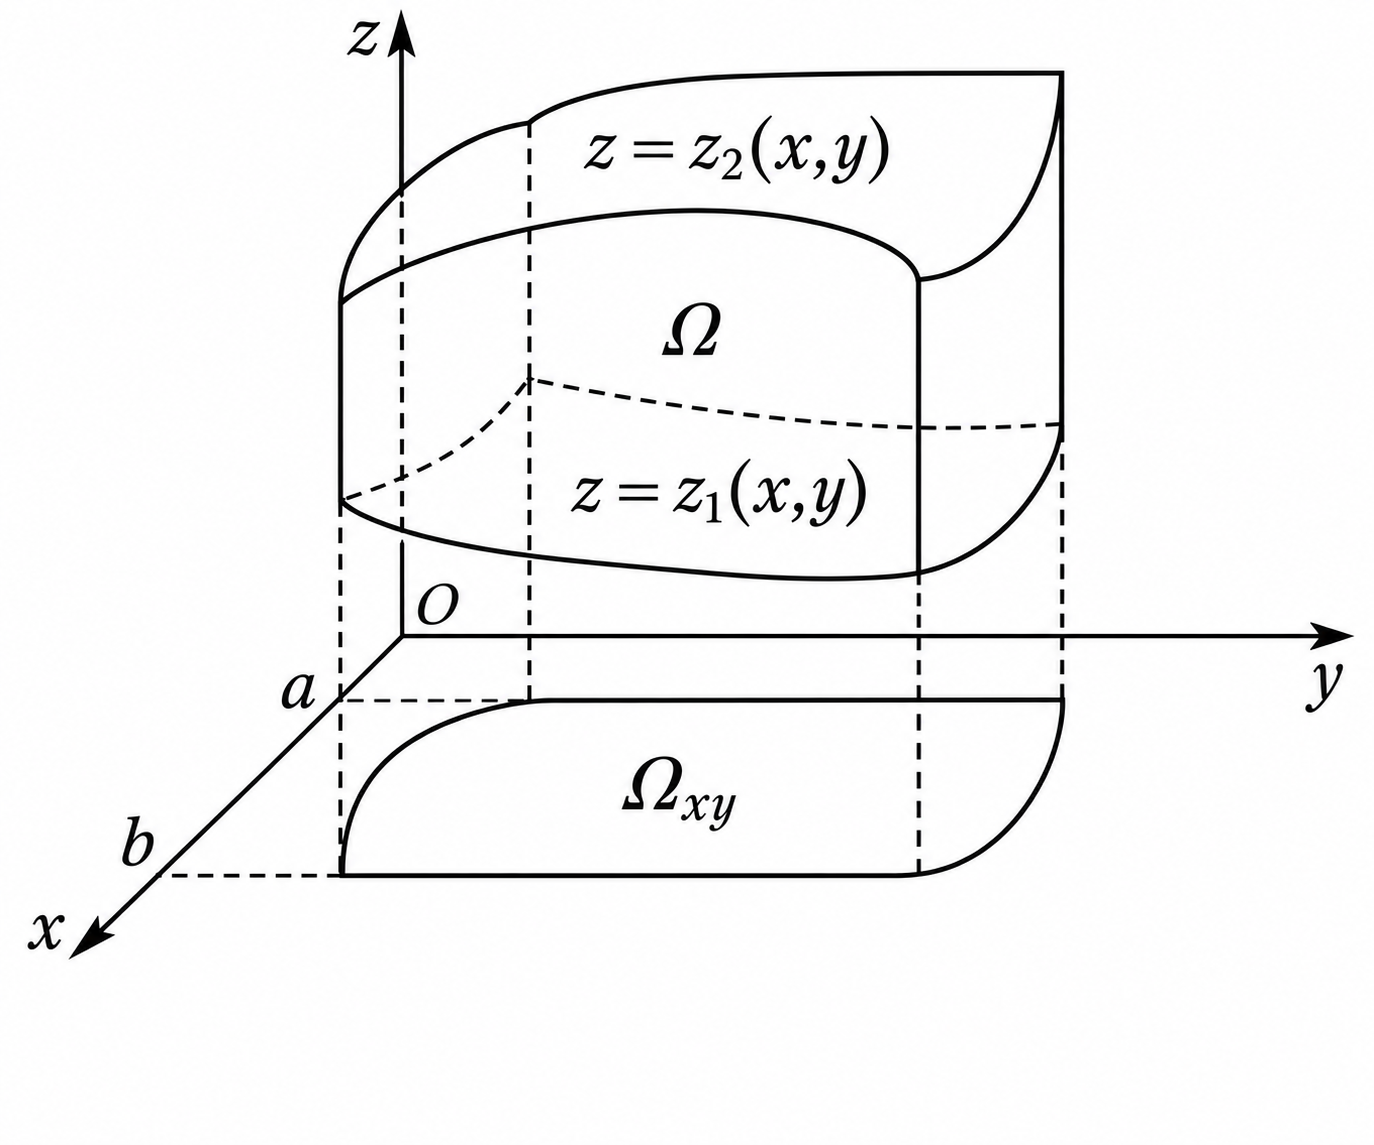
\includegraphics[width=0.5\textwidth]{figure/P2/section2_solid_hd.png}
\end{center}

\textbf{截面法：}设 $\Omega$ 夹在平面 $z=e$ 与 $z=f$ 之间，其中 $e\le f$。
固定 $z$，用平面 $z=\text{常数}$ 截取 $\Omega$，
并将所得截面投影到 $xy$ 平面，记投影区域为 $\Omega'_z$。
在相应积分存在的条件下，有
\[
\iiint_\Omega f(x,y,z)\,\dd x\,\dd y\,\dd z
=\int_e^f\dd z\iint_{\Omega'_z}f(x,y,z)\,\dd x\,\dd y.
\]
这里内层积分中的 $z$ 是固定的参数。

\begin{center}
% 截面法示意：固定 z，再把截面投影到 xy 平面。
\begin{tikzpicture}[>=Stealth,font=\small]
  \draw[line width=.6pt] (0,0) ellipse[x radius=1.35,y radius=1.15];
  \draw[dashed] (-1.35,0) arc[start angle=180,end angle=0,x radius=1.35,y radius=.24];
  \draw[line width=.6pt] (-1.35,0) arc[start angle=180,end angle=360,x radius=1.35,y radius=.24];
  \begin{scope}
    \clip (0,0) ellipse[x radius=1.35,y radius=.24];
    \foreach \s in {-1,-.6,-.2,.2,.6,1}
      \draw[thin] (\s,-.3) -- ({\s+.18},.3);
  \end{scope}
  \draw[dashed] (-1.65,1.15) -- (0,1.15);
  \draw[dashed] (-1.65,-1.15) -- (0,-1.15);
  \node[left] at (-1.65,1.15) {$z=f$};
  \node[left] at (-1.65,-1.15) {$z=e$};
  \draw[->] (2.1,.24) -- (1.1,.07);
  \node[right] at (2.1,.24) {$z=\bar z$};
\end{tikzpicture}

\end{center}

\begin{example}[非均匀金属块的质量]
一非均匀金属块在空间中的表示是由双曲抛物面 $z=xy$、
平面 $x+y=1$ 和 $z=0$ 所围成的区域 $\Omega$，
其密度函数为 $\rho(x,y,z)=xy$，求它的质量。
\end{example}
\begin{solution}
由图，$\Omega$ 可表示为
\[
\Omega=\{(x,y,z):0\le z\le xy,\ 0\le y\le1-x,\ 0\le x\le1\}.
\]

\begin{center}
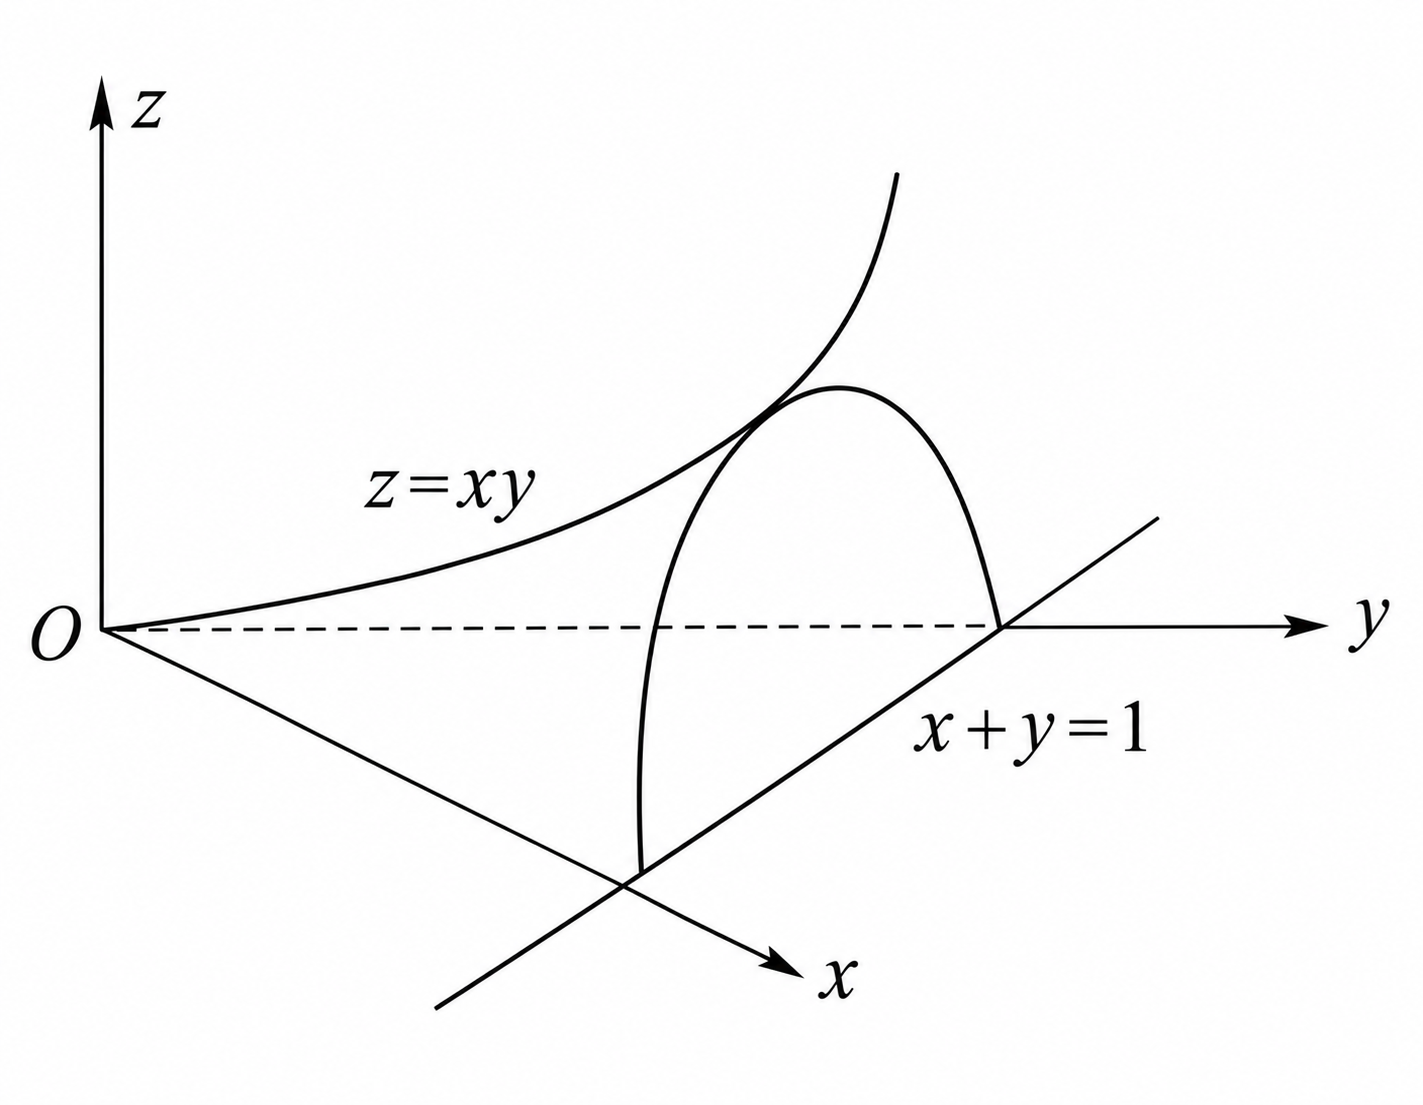
\includegraphics[width=0.45\textwidth]{figure/P2/sec2_metal_source_hd.png}
\end{center}

因此金属块的质量为
\[
\begin{aligned}
M
&=\iiint_\Omega\rho(x,y,z)\,\dd x\,\dd y\,\dd z=\int_0^1\dd x\int_0^{1-x}\dd y\int_0^{xy}xy\,\dd z=\int_0^1\dd x\int_0^{1-x}x^2y^2\,\dd y\\
&=\frac13\int_0^1x^2(1-x)^3\,\dd x=\frac13\left(\frac13-\frac34+\frac35-\frac16\right)=\frac1{180}.
\end{aligned}
\]
\end{solution}

\begin{example}[用截面法计算圆锥上的积分]
计算
\[
I=\iiint_\Omega z^2\,\dd x\,\dd y\,\dd z,
\]
其中 $\Omega$ 是由锥面
\[
z^2=\frac{h^2}{R^2}(x^2+y^2)
\]
与平面 $z=h$ 所围成的闭区域，$R>0$、$h>0$。
\end{example}
\begin{solution}
这里的 $\Omega$ 可表示为
\[
\Omega=\left\{(x,y,z):
0\le z\le h,\quad
\frac{h^2}{R^2}(x^2+y^2)\le z^2\right\}.
\]

\begin{center}
% 圆锥 z^2=(h^2/R^2)(x^2+y^2) 的上半部。
\begin{tikzpicture}[>=Stealth,font=\small,line join=round]
  \draw[->] (0,0) -- (2.2,0) node[right] {$y$};
  \draw[->] (0,0) -- (-1.25,-.95) node[below left] {$x$};
  \draw[->] (0,0) -- (0,3.35) node[above] {$z$};
  \draw[line width=.7pt] (0,0) -- (-1.05,2.55);
  \draw[line width=.7pt] (0,0) -- (1.05,2.55);
  \draw[line width=.65pt] (0,2.55) ellipse[x radius=1.05,y radius=.3];
  \node[below right] at (0,0) {$O$};
  \node[above right] at (.48,2.85) {$z=h$};
  \node[right,align=left] at (1.02,1.35)
    {$\displaystyle z^2=\frac{h^2}{R^2}(x^2+y^2)$};
\end{tikzpicture}

\end{center}

固定 $z\in[0,h]$。
用过点 $(0,0,z)$ 且平行于 $xy$ 平面的平面截取 $\Omega$，
所得截面在 $xy$ 平面上的投影为圆盘
\[
\Omega'_z
=\left\{(x,y):x^2+y^2\le\frac{R^2}{h^2}z^2\right\}.
\]
其半径为 $Rz/h$，所以
\[
\iint_{\Omega'_z}\dd x\,\dd y
=\pi\frac{R^2}{h^2}z^2.
\]

由截面法，
\[
\begin{aligned}
I
&=\int_0^h\dd z\iint_{\Omega'_z}z^2\,\dd x\,\dd y\\
&=\int_0^h z^2
\left(\iint_{\Omega'_z}\dd x\,\dd y\right)\dd z\\
&=\frac{\pi R^2}{h^2}\int_0^h z^4\,\dd z\\
&=\frac{\pi R^2h^3}{5}.
\end{aligned}
\]
\end{solution}

